%%%
%
% $Autor: Wings $
% $Datum: 2021-05-14 $
% $Dateiname: 
% $Version: 4620 $
%
% !TeX spellcheck = GB
% !TeX program = pdflatex
% !TeX encoding = utf8
%
%%%


\chapter{Package \PYTHON{Matplotlib}}

\index{Example}

\section{Introduction}

Matplotlib is a standout tool in the world of Python programming, especially when it comes to turning data into easy-to-understand visuals. Created by John D. Hunter in 2003, Matplotlib was inspired by MATLAB’s plotting capabilities, aiming to bring similar high-quality graphing tools to Python. This package stands out for its ability to handle everything from simple charts to complex graphics, making it a go-to for data analysts, scientists, and engineers.

One of Matplotlib's biggest strengths is its simplicity combined with its power. The package is designed with a philosophy that even the most basic interface should allow users to accomplish common tasks effortlessly. Yet, for more advanced needs, users don't need to start from scratch but can build on the existing framework, tweaking from minor plot adjustments to major styling overhauls. Built on top of NumPy, which is essential for numerical computations in Python, Matplotlib manages large datasets and complicated data transformations smoothly

Customization is at the heart of Matplotlib’s functionality, thanks to its layered architecture and extensive API. Whether you're adjusting the color scheme, labeling axes, or reordering layers, Matplotlib provides the tools to fine-tune every detail. This flexibility lets users craft visuals that are not only precise in conveying information but also appealing to the eye. This balance of depth and accessibility ensures that Matplotlib isn’t just a powerful tool for technical computing but also a dynamic platform for creative data visualization\cite{Yim:2018}.

For example, if you want to quickly visualize how something changes over time, you can use Matplotlib to create a line graph with just a few lines of code:

\begin{lstlisting}[language=Python, caption=Python Example: Plotting Daily Temperature]
	import matplotlib.pyplot as plt
	
	# Sample data
	time = [0, 1, 2, 3, 4, 5]  # Time in days
	temperature = [22, 24, 18, 21, 20, 19]  # Temperature in Celsius
	
	# Create a line chart
	plt.plot(time, temperature)
	plt.title('Daily Temperature Over Time')
	plt.xlabel('Time (days)')
	plt.ylabel('Temperature (Celsius)')
	plt.show()
\end{lstlisting}


%\index{Example!Introduction}


\section{Description}

Matplotlib is a fundamental tool in the data science and visualization toolkit of Python, alongside libraries like Pandas and NumPy. It offers a comprehensive range of plotting functions and extensive customization options, making it a popular choice for crafting insightful visualizations.

\subsection{Key Features of Matplotlib}

Matplotlib is renowned for its diverse capabilities in data visualization:

\begin{enumerate}
	\item \textbf{Plotting Functions:} The package supports a variety of plotting functions such as line plots, scatter plots, bar plots, histograms, pie charts, box plots, and more, facilitating different data representation needs.
	\item \textbf{Customization Options:} Users have extensive control over plot aesthetics including axes, labels, titles, colors, markers, line styles, legends, and annotations, enabling highly tailored visual presentations.
	\item \textbf{Multiple Subplots:} Matplotlib allows for multiple subplots within a single figure, useful for comparing varied datasets or aspects of data simultaneously.
	\item \textbf{3D Plotting:} The package includes capabilities for 3D visualizations, such as scatter, surface, and wireframe plots, useful for spatial and volumetric data.
	\item \textbf{Colormaps:} A broad array of built-in colormaps enhances data visualization, with support for custom color schemes to suit specific analysis needs.\cite{Matplotlib:2024}
\end{enumerate}

\subsection{Architecture}

Matplotlib's architecture is built upon three primary layers, each serving a distinct purpose in the visualization creation process:

\begin{description}
	\item[Scripting Layer (pyplot):] This layer offers a state-machine interface similar to MATLAB, facilitating quick and easy generation of plots.
	\item[Artist Layer:] Here, detailed control over plot elements is possible, ideal for creating custom visualizations.
	\item[Backend Layer:] This layer handles the rendering of figures to screens or files, supporting various output formats and environments.
\end{description}

\subsection{Integration with Other Libraries}

Matplotlib integrates well with data manipulation libraries like NumPy and pandas, enhancing its ability to handle complex data operations. This integration extends to libraries such as SciPy and scikit-learn, supporting a broad range of statistical analysis and machine learning applications.

\begin{lstlisting}[language=Python, caption=Example - Plotting Data from pandas DataFrame]
	import pandas as pd
	import matplotlib.pyplot as plt
	
	# Create a DataFrame
	data = pd.DataFrame({
		'Year': [2011, 2012, 2013, 2014],
		'Sales': [200, 250, 270, 300]
	})
	
	# Plotting directly from a DataFrame
	data.plot(x='Year', y='Sales', kind='line')
	plt.title('Yearly Sales')
	plt.ylabel('Sales')
	plt.show()
\end{lstlisting}

\subsection{Applications and Uses}

Matplotlib is utilized across various domains such as scientific computing, engineering, and data analysis, serving as a versatile tool for both simple plots and complex animations. It is essential for academics, researchers, and analysts for visual data exploration and explanatory data analysis.

\subsection{Advantages and Limitations}

\textbf{Advantages:}
\begin{itemize}
	\item \textbf{Versatility:} Suitable for a wide array of visualization tasks, from static charts to interactive plots.
	\item \textbf{Customization:} Extensive customization options allow for precise control over the visual representation of data.
	\item \textbf{Community and Support:} A robust community provides extensive documentation and support.
\end{itemize}

\textbf{Limitations:}
\begin{itemize}
	\item \textbf{Complexity:} The depth of functionality can be daunting for newcomers.
	\item \textbf{Performance:} May exhibit performance bottlenecks with very large datasets or in real-time scenarios.
\end{itemize}



\section{Installation}


Matplotlib is a powerful and versatile package in Python used for creating high-quality visualizations. It plays a crucial role in data visualization tasks, enabling users to represent complex data in a clear and informative manner. Installing Matplotlib correctly is essential for Python users as it provides access to a wide range of plotting functions and customization options, empowering them to effectively communicate insights derived from their data.

\subsection{System Requirements}
Matplotlib is compatible with major operating systems including Windows, macOS, and Linux. It supports different versions of Python, including Python 3.x. However, it's important to ensure compatibility with the specific Python version you are using to avoid compatibility issues during installation.

\subsection{Installation Methods}
There are several methods to install Matplotlib:

\begin{enumerate}[label=\arabic*.]
	\item \textbf{Using pip:} This is the most common method for installing Python packages. Pip is Python's package manager, and it can be used to install Matplotlib along with its dependencies. To install Matplotlib using pip, open a terminal or command prompt and run the following command:
	\begin{lstlisting}
		pip install matplotlib
	\end{lstlisting}
	
	\item \textbf{Using Conda:} Conda is another popular package manager, particularly for users of the Anaconda distribution. Matplotlib can be installed using Conda by running the following command:
	\begin{lstlisting}
		conda install matplotlib
	\end{lstlisting}
	
	\item \textbf{Using Package Managers:} On Linux-based systems, you can use package managers like apt for Ubuntu/Debian or brew for macOS to install Matplotlib system-wide. For example, on Ubuntu, you can install Matplotlib using apt by running:
	\begin{lstlisting}
		sudo apt-get install python3-matplotlib
	\end{lstlisting}
\end{enumerate}

\subsection*{Step-by-Step Installation Guide}
Below are detailed instructions for installing Matplotlib using pip:

\begin{enumerate}[label=\arabic*.]
	\item \textbf{Open Terminal or Command Prompt:} Navigate to your system's terminal or command prompt.
	
	\item \textbf{Install Matplotlib:} Run the following command to install Matplotlib using pip:
	\begin{lstlisting}
		pip install matplotlib
	\end{lstlisting}
	
	\item \textbf{Wait for Installation to Complete:} Pip will download and install Matplotlib along with any required dependencies. This process may take a few minutes depending on your internet connection speed.
	
	\item \textbf{Verify the Installation:} After installation, open a Python interpreter and import Matplotlib to verify that it has been installed correctly:
	\begin{lstlisting}[language=Python]
		import matplotlib.pyplot as plt
	\end{lstlisting}
	
	\item \textbf{Test Matplotlib Functionality:} Run a simple plot to ensure Matplotlib is working correctly:
	\begin{lstlisting}[language=Python]
		import matplotlib.pyplot as plt
		plt.plot([1, 2, 3, 4], [1, 4, 9, 16])
		plt.show()
	\end{lstlisting}
\end{enumerate}

\subsection{Verifying the Installation}
To verify that Matplotlib has been installed correctly, you can import it into a Python environment and check for any errors. Additionally, running a simple plot using Matplotlib's plotting functions can confirm its functionality.

\subsection{Troubleshooting}
Common errors during Matplotlib installation may include version conflicts, missing dependencies, or permission issues. Ensure that you are using the correct Python environment and try reinstalling Matplotlib. If issues persist, consult the official Matplotlib documentation or seek assistance from online forums or community channels.

\subsection{Upgrading and Uninstalling Matplotlib}
To upgrade Matplotlib to a newer version, you can use pip or Conda to install the latest release. For example, to upgrade using pip, run:
\begin{lstlisting}
	pip install --upgrade matplotlib
\end{lstlisting}
To uninstall Matplotlib, use pip or Conda to remove the package from your Python environment:
\begin{lstlisting}
	pip uninstall matplotlib
\end{lstlisting}

\subsection{Additional Resources}
For further assistance with Matplotlib installation and usage, refer to the official Matplotlib documentation available at \texttt{https://matplotlib.org/}. You can also find helpful resources and community support on platforms like Stack Overflow or the Matplotlib user mailing list.

%\index{Example!Installation}

%\SHELL{pip packageExample}


\section{Example - Basic Plotting with Matplotlib}

Matplotlib offers a simple and intuitive interface for creating plots. It provides two primary ways to create plots: the pyplot interface and the object-oriented interface. The pyplot interface provides a MATLAB-like environment for plotting, while the object-oriented interface offers more control and flexibility over the plots.\cite{Scipymatplotlib:2024}

\begin{lstlisting}[language=Python]
	import matplotlib.pyplot as plt
	
	# Using the pyplot interface
	plt.plot([1, 2, 3, 4], [1, 4, 9, 16])
	plt.show()
\end{lstlisting}

\subsection*{Creating Simple Line Plots, Scatter Plots, and Bar Plots}

\subsection{Line Plots}
Line plots are commonly used to visualize the relationship between two variables. Matplotlib makes it easy to create line plots using the \texttt{plot()} function.

\begin{lstlisting}[language=Python]
	import matplotlib.pyplot as plt
	
	x = [1, 2, 3, 4]
	y = [1, 4, 9, 16]
	
	plt.plot(x, y)
	plt.xlabel('X-axis')
	plt.ylabel('Y-axis')
	plt.title('Simple Line Plot')
	plt.show()
\end{lstlisting}

\begin{figure}[h]
	\centering
	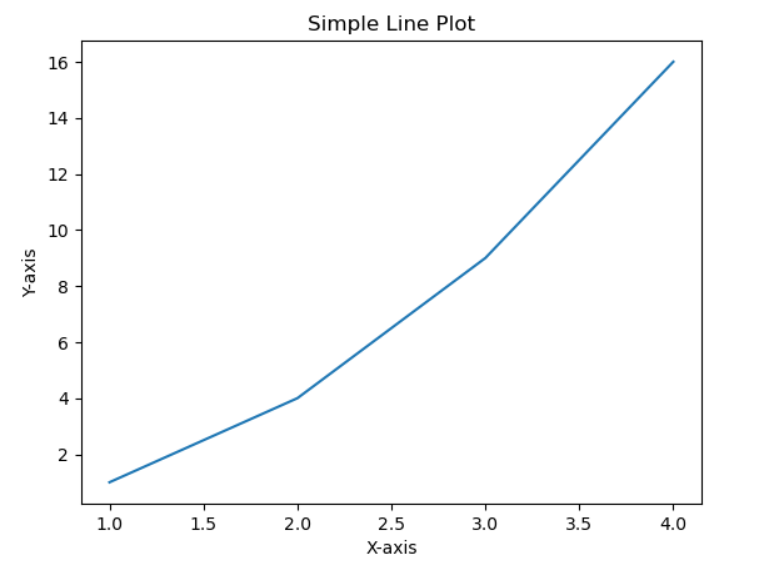
\includegraphics[width=\textwidth]{MatPlotLib/MatPlotLib101}
	\caption{Simple Line Plot}\label{Matplotlib01}
\end{figure}

\subsection{Scatter Plots}
Scatter plots are useful for visualizing the distribution and relationship between two variables. Matplotlib provides the \PYTHON{scatter()} function to create scatter plots.

\begin{lstlisting}[language=Python]
	import matplotlib.pyplot as plt
	
	x = [1, 2, 3, 4]
	y = [1, 4, 9, 16]
	
	plt.scatter(x, y)
	plt.xlabel('X-axis')
	plt.ylabel('Y-axis')
	plt.title('Scatter Plot')
	plt.show()
\end{lstlisting}

\begin{figure}[h]
	\centering
	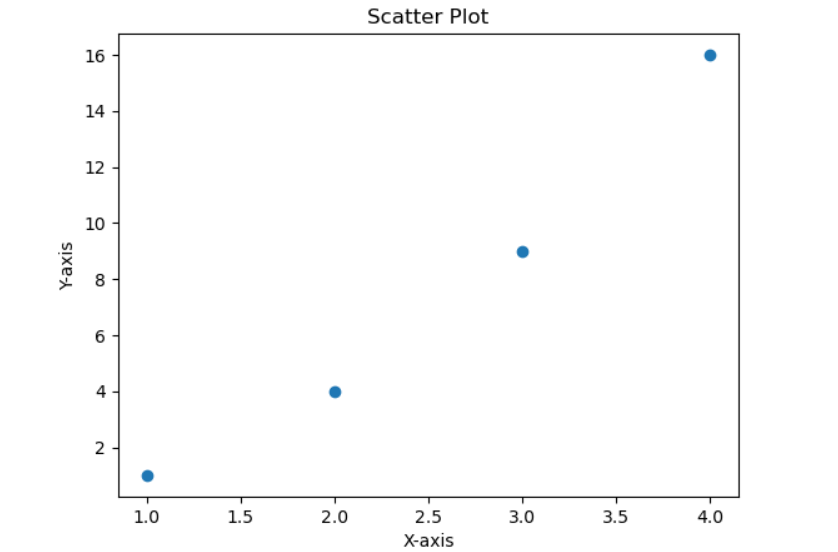
\includegraphics[width=\textwidth]{MatPlotLib/MatPlotLib102}
	\caption{Scatter Plot}\label{Matplotlib02}
\end{figure}

\subsection{Bar Plots}
Bar plots are effective for comparing categorical data. Matplotlib allows you to create bar plots using the \PYTHON{bar()} function. \cite{Scipymatplotlib:2024}

\begin{lstlisting}[language=Python]
	import matplotlib.pyplot as plt
	
	categories = ['A', 'B', 'C', 'D']
	values = [3, 7, 2, 5]
	
	plt.bar(categories, values)
	plt.xlabel('Categories')
	plt.ylabel('Values')
	plt.title('Bar Plot')
	plt.show()
\end{lstlisting}

\begin{figure}[h]
	\centering
	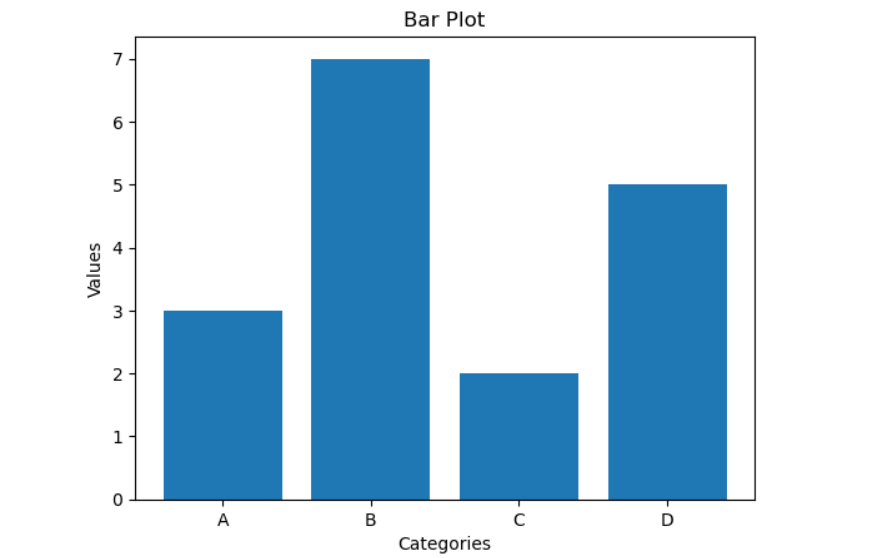
\includegraphics[width=\textwidth]{MatPlotLib/MatPlotLib103}
	\caption{Bar Plot}\label{Matplotlib03}
\end{figure}

\subsection*{Customizing Plot Appearance}

Matplotlib provides extensive customization options to enhance the appearance of plots.

\subsection*{Colors}
You can specify colors using named colors, hex RGB codes, or RGB tuples.

\begin{lstlisting}[language=Python]
	plt.plot(x, y, color='green')
	plt.scatter(x, y, color='#FF5733')
	plt.bar(categories, values, color=('blue', 'red', 'green', 'yellow'))
\end{lstlisting}

\subsection*{Labels, Titles, and Legends}
You can add labels to axes, titles to plots, and legends to identify plotted data.

\begin{lstlisting}[language=Python]
	plt.xlabel('X-axis')
	plt.ylabel('Y-axis')
	plt.title('Plot Title')
	plt.legend(['Line'], loc='upper left')
\end{lstlisting}

\begin{figure}[h]
	\centering
	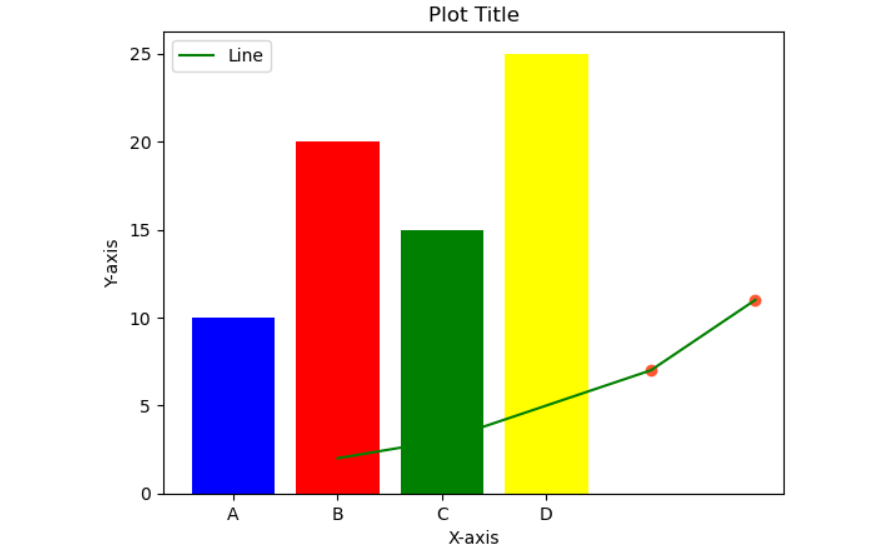
\includegraphics[width=\textwidth]{MatPlotLib/MatPlotLib104}
	\caption{Labels, Titles, and Legends}\label{Matplotlib04}
\end{figure}


\section*{Setting Limits}

Setting limits in Matplotlib allows you to control the range of values displayed along the x and y axes. This is particularly useful when you want to focus on a specific range of data or when you need to emphasize certain aspects of your plot.

\begin{lstlisting}
	import matplotlib.pyplot as plt
	import numpy as np
	
	x = np.linspace(0, 10, 100)
	y = np.sin(x)
	
	plt.plot(x, y)
	plt.xlim(0, 5)  # set x-axis limits
	plt.ylim(-1, 1) # set y-axis limits
	plt.show()
\end{lstlisting}

In this example, \PYTHON{plt.xlim()} and \PYTHON{plt.ylim()} are used to set the limits for the x and y axes, respectively, restricting the displayed range of the plot.

\begin{figure}[h]
	\centering
	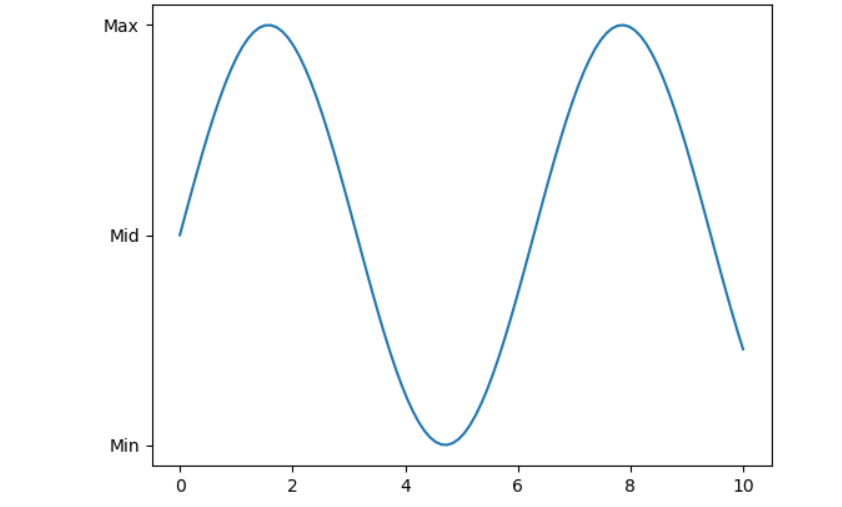
\includegraphics[width=\textwidth]{MatPlotLib/MatPlotLib105}
	\caption{Setting Ticks}\label{Matplotlib05}
\end{figure}

\section*{Setting Ticks}

Ticks are the markers denoting specific data points on the axes. You can customize these ticks to better represent your data or make your plot more readable.

\begin{lstlisting}
	import matplotlib.pyplot as plt
	import numpy as np
	
	x = np.linspace(0, 10, 100)
	y = np.sin(x)
	
	plt.plot(x, y)
	plt.xticks(np.arange(0, 11, 2))  # set custom ticks on x-axis
	plt.yticks([-1, 0, 1], ['Min', 'Mid', 'Max']) # set custom ticks and labels on y-axis
	plt.show()
\end{lstlisting}

Here, \PYTHON{plt.xticks()} and \PYTHON{plt.yticks()} allow you to specify the locations and labels for ticks on the x and y axes, respectively, providing more control over the appearance of your plot.

\section*{Setting Tick Labels}

Tick labels are the textual representations of the tick marks on the axes. You can customize these labels to convey additional information or improve the clarity of your plot.

\begin{lstlisting}
	import matplotlib.pyplot as plt
	import numpy as np
	
	x = np.linspace(0, 10, 100)
	y = np.sin(x)
	
	plt.plot(x, y)
	plt.xticks(np.arange(0, 11, 2), rotation=45)  # rotate x-axis tick labels by 45 degrees
	plt.yticks([-1, 0, 1], ['Min', 'Mid', 'Max']) # set custom ticks and labels on y-axis
	plt.show()
\end{lstlisting}

In this example, \PYTHON{plt.xticks()} is used to set custom tick labels on the x-axis, and the \PYTHON{rotation} parameter rotates the labels for better readability.

\section*{Moving Spines}

Spines are the lines connecting the axis tick marks. You can adjust their position to emphasize certain aspects of your plot or create a more aesthetically pleasing visualization.

\begin{lstlisting}
	import matplotlib.pyplot as plt
	import numpy as np
	
	x = np.linspace(0, 10, 100)
	y = np.sin(x)
	
	plt.plot(x, y)
	ax = plt.gca()
	ax.spines['top'].set_visible(False)  # remove top spine
	ax.spines['right'].set_color('red')  # change color of right spine
	plt.show()
\end{lstlisting}

In this example, \texttt{ax.spines} allows you to access and customize the properties of the spines. You can remove spines (\PYTHON{set\_visible(False)}), change their color, style, or width to suit your plot's requirements.

\begin{figure}[h]
	\centering
	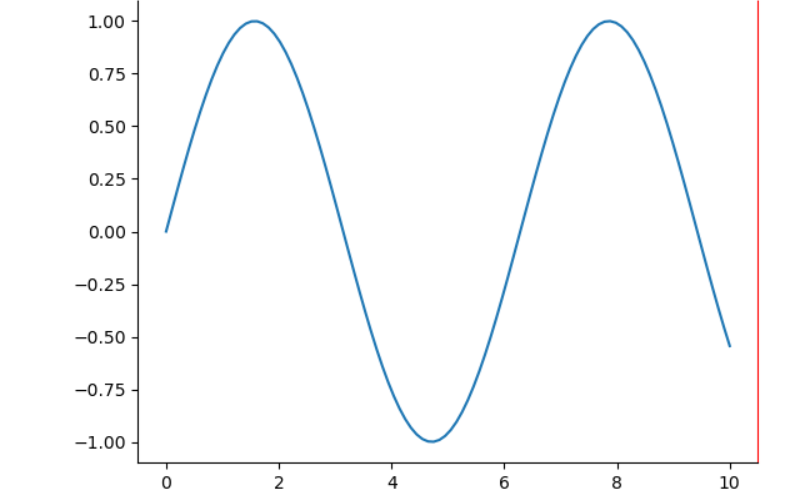
\includegraphics[width=\textwidth]{MatPlotLib/MatPlotLib106}
	\caption{Moving Spines}\label{Matplotlib06}
\end{figure}


\section*{Adding a Legend}

Legends provide information about the data represented in the plot. Adding a legend is essential when you have multiple datasets plotted on the same axes.

\begin{lstlisting}
import matplotlib.pyplot as plt

# Sample data
x = [1, 2, 3, 4, 5]
y1 = [2, 3, 5, 7, 11]
y2 = [1, 4, 6, 8, 10]
y3 = [3, 5, 7, 9, 12]

# Plotting data
plt.plot(x, y1, label='Dataset 1')
plt.plot(x, y2, label='Dataset 2')
plt.plot(x, y3, label='Dataset 3')

# Adding legend
plt.legend()

# Adding labels and title
plt.xlabel('X-axis')
plt.ylabel('Y-axis')
plt.title('Multiple Legends Example')

# Show plot
plt.show()

\end{lstlisting}

\begin{figure}[h]
	\centering
	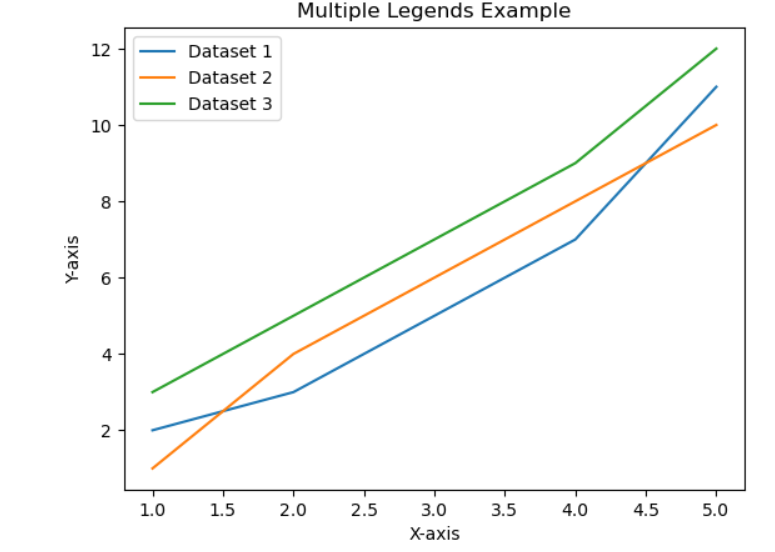
\includegraphics[width=\textwidth]{MatPlotLib/MatPlotLib107}
	\caption{Adding a Legend}\label{Matplotlib07}
\end{figure}


\section{Example - Advanced Plotting Techniques in Matplotlib}

\subsection{Subplots: Creating multiple plots in a single figure}

\textbf Subplots are a fundamental aspect of data visualization, allowing users to present multiple plots within a single figure, facilitating comparison and analysis across different datasets or aspects of the same dataset. Matplotlib provides a convenient way to create subplots through its \PYTHON{subplot()} function.

\textbf{Implementation:} To create subplots, you can use the \PYTHON{plt.subplot()} function, which takes three arguments: the number of rows, the number of columns, and the index of the subplot you want to create. \cite{Scipymatplotlib:2024} For example:

\begin{lstlisting}[language=Python]
	import matplotlib.pyplot as plt
	
	# Creating a figure with 2x2 subplots
	plt.figure(figsize=(10,8))
	
	# Creating the first subplot
	plt.subplot(2, 2, 1)
	plt.plot([1, 2, 3], [1, 2, 3])
	plt.title('Subplot 1')
	
	# Creating the second subplot
	plt.subplot(2, 2, 2)
	plt.plot([1, 2, 3], [3, 2, 1])
	plt.title('Subplot 2')
	
	# Creating the third subplot
	plt.subplot(2, 2, 3)
	plt.plot([1, 2, 3], [2, 3, 1])
	plt.title('Subplot 3')
	
	# Creating the fourth subplot
	plt.subplot(2, 2, 4)
	plt.plot([1, 2, 3], [1, 3, 2])
	plt.title('Subplot 4')
	
	plt.tight_layout()
	plt.show()
\end{lstlisting}

In this example, we create a 2x2 grid of subplots and plot different datasets on each subplot.

\begin{figure}[h]
	\centering
	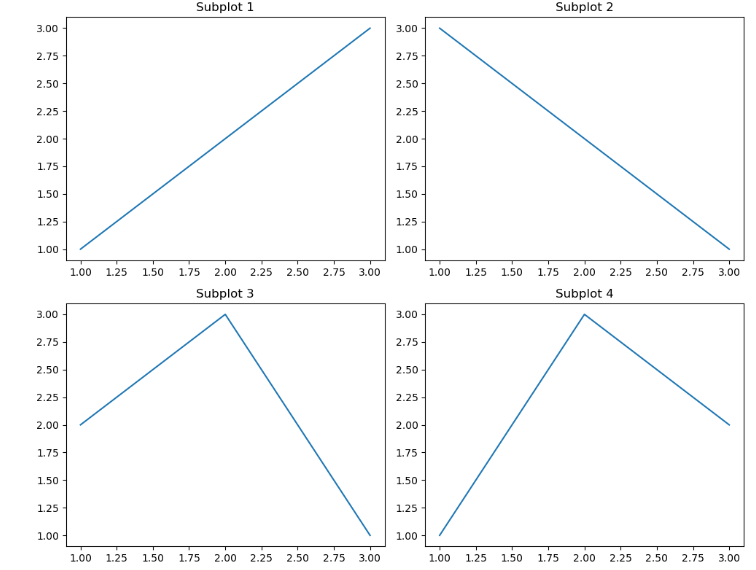
\includegraphics[width=\textwidth]{MatPlotLib/MatPlotLib108}
	\caption{Subplots}\label{Matplotlib08}
\end{figure}

\textbf{Benefits:}
\begin{itemize}
	\item Subplots allow for clear organization and comparison of multiple plots within the same figure.
	\item They enable efficient use of space, especially when presenting related visualizations.
\end{itemize}

\subsection{Annotations and text placement}

\textbf Annotations and text placement play a crucial role in communicating insights and highlighting key aspects of visualizations. Matplotlib provides various functions for adding annotations and text to plots.

\textbf{Implementation:} Matplotlib offers the \PYTHON{annotate()} function to add annotations to specific points on a plot. It takes parameters such as the text to display, the position of the annotation, and optional arrow properties. Additionally, the \PYTHON{text()} function can be used to add text at any location on the plot.

\begin{lstlisting}[language=Python]
	import matplotlib.pyplot as plt
	
	# Creating a simple plot
	plt.plot([1, 2, 3], [1, 2, 3])
	
	# Adding annotation
	plt.annotate('Important Point', xy=(2, 2), xytext=(2.5, 2.5),
	arrowprops=dict(facecolor='black', shrink=0.05))
	
	# Adding text
	plt.text(1, 1.5, 'Additional Information', fontsize=12)
	
	plt.show()
\end{lstlisting}

In this example, we annotate a specific point on the plot and add additional text.

\begin{figure}[h]
	\centering
	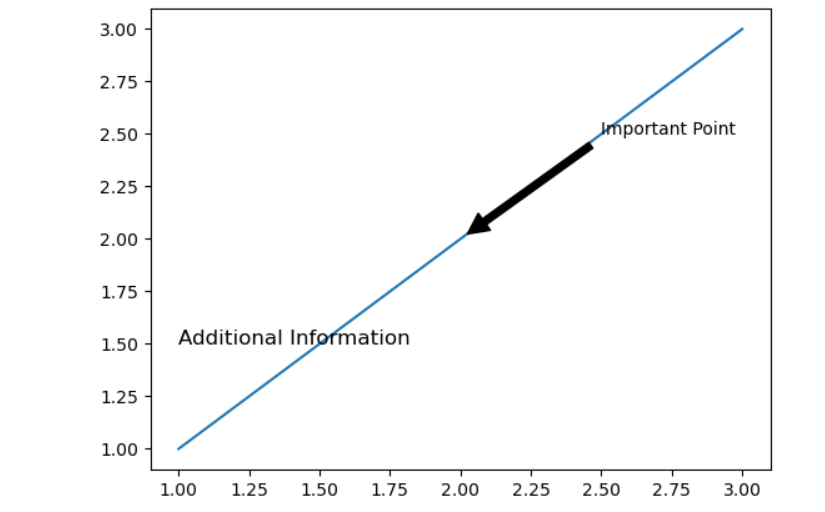
\includegraphics[width=\textwidth]{MatPlotLib/MatPlotLib109}
	\caption{Annotations and text placement}\label{Matplotlib09}
\end{figure}

\textbf{Benefits:}
\begin{itemize}
	\item Annotations provide contextual information about specific data points or trends.
	\item Text placement allows for the inclusion of supplementary details within the plot.
\end{itemize}

\subsection*{Working with different plot styles and themes}

\textbf Matplotlib offers flexibility in customizing the appearance of plots through different styles and themes. This enables users to create visually appealing and coherent visualizations that suit their preferences or the requirements of a specific audience.

\textbf{Implementation:} Matplotlib provides a variety of built-in styles and themes that can be easily applied to plots using the \PYTHON{plt.style.use()} function. Additionally, custom styles can be created and applied to achieve a unique aesthetic.

\begin{lstlisting}[language=Python]
	import matplotlib.pyplot as plt
	
	# Using a predefined style
	plt.style.use('ggplot')
	
	# Creating a plot
	plt.plot([1, 2, 3], [1, 2, 3])
	plt.title('Example Plot')
	
	plt.show()
\end{lstlisting}

In this example, we apply the 'ggplot' style to the plot, which changes the color scheme and overall appearance.

\textbf{Benefits:}
\begin{itemize}
	\item Different plot styles and themes allow for customization to match the desired visual presentation.
	\item Consistent styling across multiple plots enhances the overall coherence of visualizations.
\end{itemize}

\subsection{Figures and Axes}

\textbf In Matplotlib, figures and axes are fundamental components of a plot. Understanding their roles and relationships is essential for creating and customizing visualizations effectively.

\textbf{Implementation:} A figure in Matplotlib represents the entire window or page where the plot appears. Axes are the individual plotting areas within the figure where data is plotted. Multiple axes can exist within a single figure, allowing for complex layouts. \cite{Scipymatplotlib:2024}

\begin{lstlisting}[language=Python]
	import matplotlib.pyplot as plt
	
	# Creating a figure and axes
	fig, ax = plt.subplots()
	
	# Plotting data on the axes
	ax.plot([1, 2, 3], [1, 2, 3])
	
	# Customizing axes labels
	ax.set_xlabel('X-axis')
	ax.set_ylabel('Y-axis')
	
	# Adding a title to the plot
	ax.set_title('Example Plot')
	
	plt.show()
\end{lstlisting}

In this example, we create a figure with a single set of axes and plot data on it.

\textbf{Benefits:}
\begin{itemize}
	\item Figures provide a container for organizing and displaying plots.
	\item Axes facilitate the plotting of data and customization of various plot elements.
\end{itemize}

\section{Example - Other Types of Plots}

\subsection{Histograms}

Histograms are graphical representations of the distribution of numerical data. They consist of a series of adjacent rectangles, or bins, whose heights represent the frequency or probability of occurrences within each interval. Histograms are commonly used to visualize the distribution of data and identify patterns or outliers.

Let's say we have a dataset containing the ages of students in a class. We can create a histogram to visualize the distribution of ages, with bins representing age ranges (e.g., 10-20, 20-30, etc.) and the height of each bin representing the number of students in that age range.

\subsection*{Generate data and plot a simple histogram}

To create a simple histogram in Python using matplotlib, we first need to import the necessary libraries and generate some sample data. Then, we use the \lstinline{plt.hist()} function to plot the histogram.

\begin{lstlisting}[caption={Generate data and plot a simple histogram}, label={lst:simple_histogram}]
	import matplotlib.pyplot as plt
	import numpy as np
	
	# Generate random data
	data = np.random.normal(loc=0, scale=1, size=1000)
	
	# Plot histogram
	plt.hist(data, bins=30, color='blue', alpha=0.7)
	plt.xlabel('Value')
	plt.ylabel('Frequency')
	plt.title('Histogram of Random Data')
	plt.show()
\end{lstlisting}

\begin{figure}[h]
	\centering
	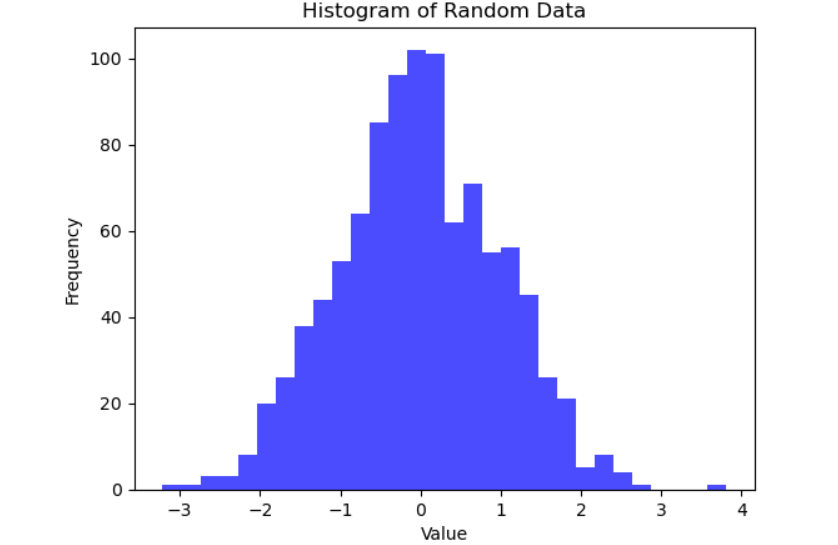
\includegraphics[width=\textwidth]{MatPlotLib/MatPlotLib110}
	\caption{Generate data and plot a simple histogram}\label{Matplotlib110}
\end{figure}

\subsection*{Updating histogram colors}

You can customize the colors of the histogram bars by specifying the color parameter in the \lstinline{plt.hist()} function.

\begin{lstlisting}[caption={Updating histogram colors}, label={lst:histogram_colors}]
	plt.hist(data, bins=30, color='green', alpha=0.5)
\end{lstlisting}

\subsection*{Plot a 2D histogram}

A 2D histogram is useful when you have two sets of data and want to visualize their joint distribution. This can be achieved using the \lstinline{plt.hist2d()} function.

\begin{lstlisting}[caption={Plot a 2D histogram}, label={lst:2d_histogram}]
	x = np.random.randn(1000)
	y = np.random.randn(1000)
	plt.hist2d(x, y, bins=30, cmap='Blues')
	plt.colorbar(label='Frequency')
	plt.xlabel('X-axis')
	plt.ylabel('Y-axis')
	plt.title('2D Histogram')
	plt.show()
\end{lstlisting}

\subsection*{Customizing your histogram}

You can customize various aspects of the histogram, such as title, labels, grid, and more using matplotlib's built-in functions and parameters.\cite{Matplotlib:2024}

\begin{lstlisting}[caption={Customizing your histogram}, label={lst:custom_histogram}]
	plt.hist(data, bins=30, color='red', alpha=0.6)
	plt.xlabel('Value')
	plt.ylabel('Frequency')
	plt.title('Customized Histogram')
	plt.grid(True, linestyle='--', alpha=0.5)
	plt.xlim(-3, 3)
	plt.ylim(0, 100)
	plt.show()
\end{lstlisting}

\subsection{Pie Charts}

Pie charts are circular statistical graphics that are divided into slices to illustrate numerical proportions. They are commonly used to represent the composition of a categorical variable.

Consider a survey where respondents were asked about their favorite fruits. We can create a pie chart to visualize the proportion of respondents who chose each fruit.\cite{Tosi:2009}

\subsection*{Label slices}

You can label each slice of the pie chart with its corresponding category using the \PYTHON{plt.pie()} function's \PYTHON{labels} parameter.

\begin{lstlisting}[language=Python]
	import matplotlib.pyplot as plt
	
	labels = ['Apple', 'Banana', 'Orange', 'Grapes']
	sizes = [30, 20, 25, 25]
	plt.pie(sizes, labels=labels)
	plt.show()
\end{lstlisting}

\subsection*{Auto-label slices}

By default, matplotlib automatically labels each slice with its percentage of the total. You can disable this feature by setting the \texttt{autopct} parameter to an empty string.

\begin{lstlisting}[language=Python]
	plt.pie(sizes, labels=labels, autopct='')
\end{lstlisting}

\subsection*{Color slices, Hatch slices}

You can customize the colors and hatch patterns of the slices using the \texttt{colors} and \texttt{hatch} parameters, respectively.

\begin{lstlisting}[language=Python]
	colors = ['red', 'green', 'blue', 'yellow']
	hatches = ['/', '\\', '|', '-']
	plt.pie(sizes, labels=labels, colors=colors, autopct='%1.1f%%', startangle=90, pctdistance=0.85, explode=(0, 0.1, 0, 0))
\end{lstlisting}


\begin{figure}[h]
	\centering
	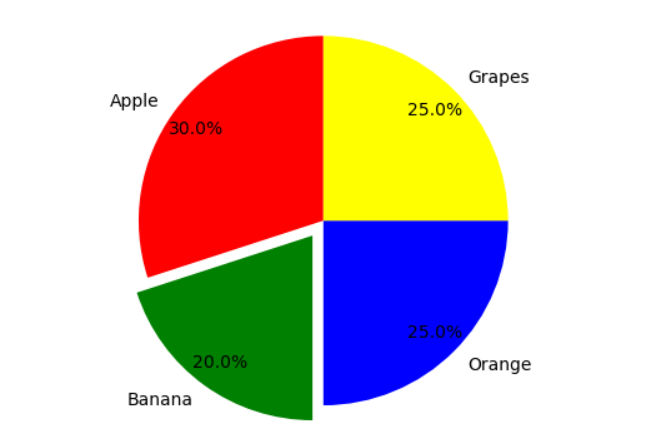
\includegraphics[width=\textwidth]{MatPlotLib/MatPlotLib111}
	\caption{Pie Chart- Color slices and Hatch slices}\label{Matplotlib111}
\end{figure}

\subsection*{Swap label and autopct text positions}

You can swap the positions of the slice labels and autopct text by setting the \texttt{labeldistance} parameter to 0 and adjusting the \texttt{pctdistance}.

\begin{lstlisting}[language=Python]
	plt.pie(sizes, labels=labels, autopct='%1.1f%%', startangle=90, pctdistance=0.5, labeldistance=0.75)
\end{lstlisting}

\subsection*{Explode, shade, and rotate slices}

You can explode (pull out) specific slices, shade them, and rotate the entire pie chart using various parameters such as \texttt{explode}, \texttt{shadow}, and \texttt{startangle}.

\begin{lstlisting}[language=Python]
	explode = (0, 0.1, 0, 0)
	plt.pie(sizes, labels=labels, explode=explode, shadow=True, startangle=90)
\end{lstlisting}

\subsection*{Controlling the size, Modifying the shadow}

You can control the size of the pie chart using the \texttt{figsize} parameter in \PYTHON{plt.figure()}. Additionally, you can modify the shadow effect using the \texttt{shadow} parameter.

\begin{lstlisting}[language=Python]
	plt.figure(figsize=(8, 8))
	plt.pie(sizes, labels=labels, shadow=False)
\end{lstlisting}


\subsection{Density Plots}

Density plots, also known as kernel density plots, provide a smooth estimation of the probability density function of a continuous random variable. They are particularly useful when visualizing the distribution of data, especially when histograms might not provide enough detail due to binning. \cite{Tosi:2009}

\subsection*{Generating a Density Plot}

Let's consider a dataset of exam scores. We can use Seaborn, a Python data visualization package built on top of Matplotlib, to generate a density plot:

\begin{lstlisting}[language=Python, caption={Generating a Density Plot}]
import matplotlib.pyplot as plt
import numpy as np

# Generate random exam scores
np.random.seed(0)
scores = np.random.normal(loc=70, scale=15, size=100)

# Plot density plot
plt.figure(figsize=(8, 6))
plt.hist(scores, bins=20, density=True, color='blue', alpha=0.7)
plt.title('Density Plot of Exam Scores')
plt.xlabel('Scores')
plt.ylabel('Density')
plt.grid(True)
plt.show()
\end{lstlisting}


\begin{figure}[h]
	\centering
	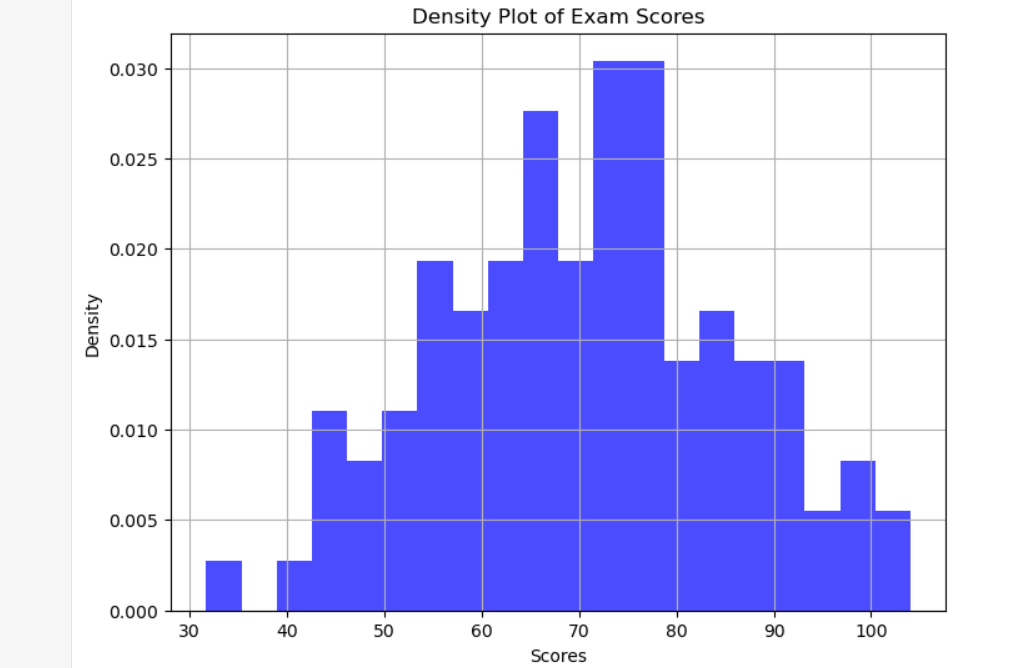
\includegraphics[width=\textwidth]{MatPlotLib/MatPlotLib112}
	\caption{Generating a Density Plot}\label{Matplotlib112}
\end{figure}

This code generates 100 random exam scores with a mean of 70 and a standard deviation of 15, then plots the density plot using Seaborn's 'kdeplot' function. The 'shade' parameter fills the area under the curve with the specified color.

\subsection*{Customizing Density Plot}

You can customize various aspects of a density plot, such as the line style, bandwidth, and color palette. For example, let's change the line style to dashed and set a different color palette:

\begin{lstlisting}[language=Python, caption={Customizing Density Plot}]
	sns.kdeplot(scores, linestyle='--', color='green', bw_adjust=0.5)
\end{lstlisting}

This code modifies the density plot to have dashed lines with a green color, and adjusts the bandwidth of the kernel density estimation using the 'bw\_adjust' parameter.

\subsection*{Interpreting Density Plot}

Density plots provide a smooth representation of the distribution of data, making it easier to identify patterns such as multimodal distributions or skewness. They are particularly useful for comparing distributions between different groups or conditions.

\subsection{Box Plots}

Box plots, also known as box-and-whisker plots, are a standardized way of displaying the distribution of data based on the five-number summary: minimum, first quartile, median, third quartile, and maximum. They are excellent tools for detecting outliers and comparing distributions.

\subsection*{Generating a Box Plot}

Let's use Seaborn to generate a box plot for the exam scores dataset:

\begin{lstlisting}[language=Python, caption={Generating a Box Plot}]
	sns.boxplot(y=scores, color='skyblue')
\end{lstlisting}

This code creates a box plot for the exam scores, with the y-axis representing the scores. The boxes extend from the lower to upper quartile values of the data, with a line at the median. The whiskers extend from the edges of the box to show the range of the data, excluding outliers.

\subsection*{Interpreting Box Plot}

Box plots provide a visual summary of the central tendency, spread, and skewness of a dataset. They are particularly useful for identifying outliers and comparing distributions between different groups or conditions.

\subsection*{Customizing Box Plot}

You can customize various aspects of a box plot, such as the color, width, and style of the boxes and whiskers. For example, let's change the width of the boxes and set a different color:

\begin{lstlisting}[language=Python, caption={Customizing Box Plot}]
	sns.boxplot(y=scores, width=0.2, color='orange')
\end{lstlisting}

This code modifies the box plot to have narrower boxes with an orange color, making it easier to distinguish between different conditions or groups.

\begin{figure}[h]
	\centering
	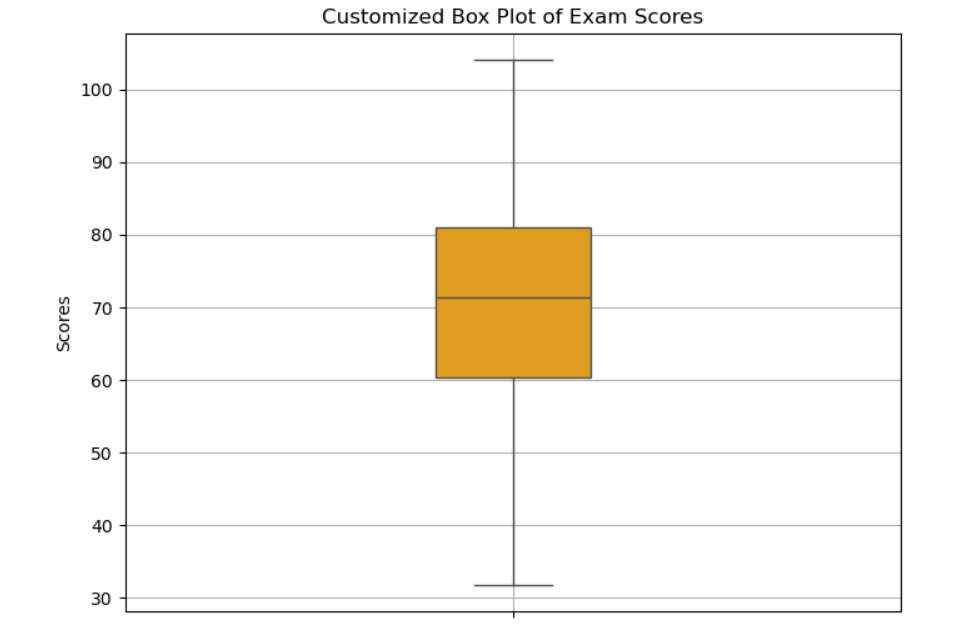
\includegraphics[width=\textwidth]{MatPlotLib/MatPlotLib113}
	\caption{Customizing Box Plot}\label{Matplotlib113}
\end{figure}

\subsection{Violin Plots}

Violin plots combine the benefits of box plots and kernel density plots by displaying both the summary statistics of a dataset and its underlying probability density distribution. They provide a more detailed summary of the distribution compared to box plots alone.

\subsection*{Generating a Violin Plot}

Let's generate a violin plot for the exam scores dataset using Seaborn:

\begin{lstlisting}[language=Python, caption={Generating a Violin Plot}]
	sns.violinplot(y=scores, color='purple')
\end{lstlisting}

\begin{figure}[h]
	\centering
	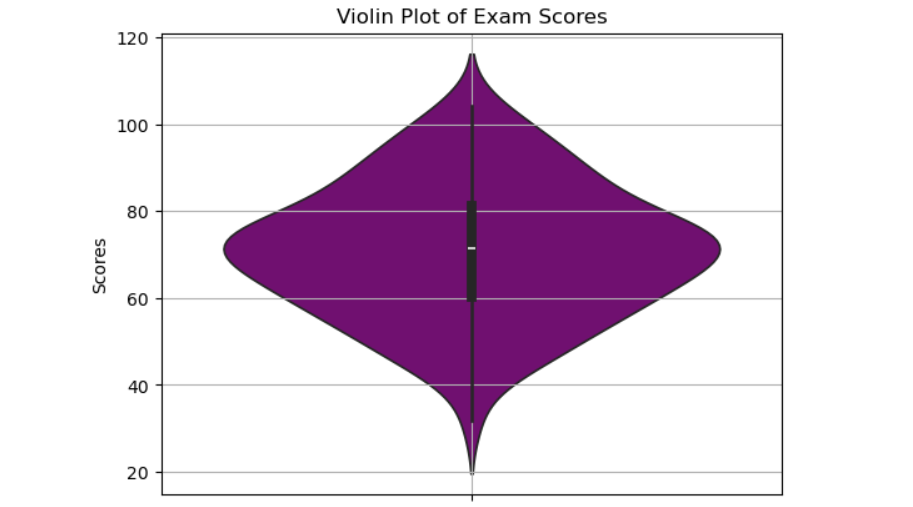
\includegraphics[width=\textwidth]{MatPlotLib/MatPlotLib114}
	\caption{Generating a Violin Plot}\label{Matplotlib114}
\end{figure}

This code creates a violin plot for the exam scores, with the y-axis representing the scores. The width of the violin represents the density of the data at different values, with the white dot indicating the median.

\subsection*{Interpreting Violin Plot}

Violin plots provide a visual summary of the distribution of data, including information about the central tendency, spread, and multi modality. They are particularly useful for comparing distributions between different groups or conditions.

\subsection*{Customizing Violin Plot}

You can customize various aspects of a violin plot, such as the width, color, and bandwidth of the kernel density estimation. For example, let's increase the width of the violin and set a different color:

\begin{lstlisting}[language=Python, caption={Customizing Violin Plot}]
	sns.violinplot(y=scores, width=0.5, color='green')
\end{lstlisting}

This code modifies the violin plot to have wider violins with a green color, providing a clearer representation of the distribution of data.

\subsection*{Polar Plots}

Polar plots, also known as radial plots or polar charts, are graphical representations of data in a two-dimensional coordinate system where each point is determined by a distance from a reference point and an angle from a reference direction. They are particularly useful for visualizing cyclic or periodic data, such as direction, frequency, or time. \cite{Tosi:2009}

To illustrate how to create a polar plot, let's consider a dataset representing wind speed and direction over time. We'll generate synthetic data and plot it using Matplotlib:

\begin{lstlisting}[language=Python]
	import matplotlib.pyplot as plt
	import numpy as np
	
	# Generate synthetic wind speed and direction data
	time = np.linspace(0, 2*np.pi, 100)
	wind_speed = 10 + 5 * np.sin(2*time)
	wind_direction = np.rad2deg(time)
	
	# Plot polar plot
	plt.figure(figsize=(8, 8))
	plt.polar(np.deg2rad(wind_direction), wind_speed)
	plt.title('Wind Speed and Direction')
	plt.show()
\end{lstlisting}

In this example, we use NumPy to generate synthetic wind speed data varying sinusoidally over time and corresponding wind directions. Then, we plot these data in a polar coordinate system using Matplotlib's \PYTHON{plt.polar()} function. The wind direction is represented by the angle from the reference direction (usually North), and the wind speed determines the distance from the center.

\section*{Customizing Polar Plots}

You can customize various aspects of a polar plot, such as the line style, marker style, labels, and gridlines. For instance, let's modify the line color and add gridlines:

\begin{lstlisting}[language=Python]
	plt.polar(np.deg2rad(wind_direction), wind_speed, color='green', marker='o', linestyle='--')
	plt.grid(True)
\end{lstlisting}

This code changes the line color to green, sets markers at data points, and adds circular gridlines to the polar plot.

\section*{Plotting Multiple Data Series}

Polar plots can visualize multiple data series simultaneously, making it easier to compare different datasets. For example, let's overlay two wind speed profiles representing different weather conditions:

\begin{lstlisting}[language=Python]
	wind_speed_2 = 8 + 6 * np.sin(2*time)
	
	plt.polar(np.deg2rad(wind_direction), wind_speed, label='Condition A')
	plt.polar(np.deg2rad(wind_direction), wind_speed_2, label='Condition B')
	plt.legend()
\end{lstlisting}

\begin{figure}[h]
	\centering
	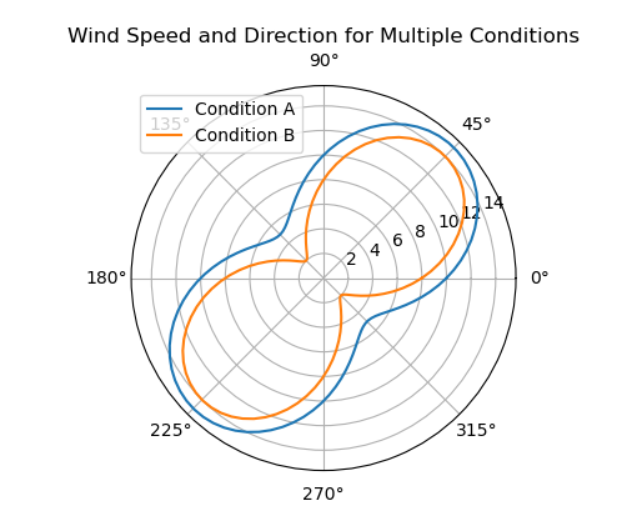
\includegraphics[width=\textwidth]{MatPlotLib/MatPlotLib115}
	\caption{Wind Speed and Direction for Multiple Conditions}\label{Matplotlib115}
\end{figure}

Here, we generate another set of wind speed data (\PYTHON{wind\_speed\_2}) for a different condition and overlay it with the previous data. Adding a legend helps distinguish between the two conditions.

\subsection{3D Plots}

3D plots, or three-dimensional plots, are graphical representations of data that involve three axes: \(x\), \(y\), and \(z\). They are useful for visualizing complex relationships and spatial data in a more intuitive manner.

\subsection*{Surface Plot}

One common type of 3D plot is the surface plot, which displays a three-dimensional surface over a rectangular grid. Let's generate and visualize a surface plot of a mathematical function, such as the Rosenbrock function:

\begin{lstlisting}[language=Python]
	from mpl_toolkits.mplot3d import Axes3D
	
	fig = plt.figure()
	ax = fig.add_subplot(111, projection='3d')
	
	x = np.linspace(-5, 5, 100)
	y = np.linspace(-5, 5, 100)
	x, y = np.meshgrid(x, y)
	z = (1-x)**2 + 100*(y-x**2)**2
	
	ax.plot_surface(x, y, z, cmap='viridis')
	ax.set_title('Surface Plot of Rosenbrock Function')
	plt.show()
\end{lstlisting}

In this example, we use Matplotlib's \texttt{Axes3D} to create a 3D subplot. We define the \(x\) and \(y\) coordinates as a meshgrid spanning a range, calculate the corresponding \(z\) values based on the Rosenbrock function, and then plot the surface using \PYTHON{ax.plot\_surface()}.

\begin{figure}[h]
	\centering
	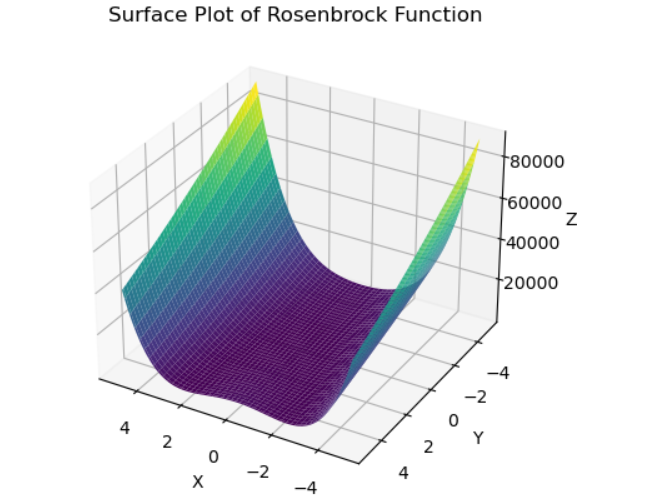
\includegraphics[width=\textwidth]{MatPlotLib/MatPlotLib116}
	\caption{Surface Plot of Rosenbrock Function}\label{Matplotlib116}
\end{figure}

\section*{Customizing 3D Plots}

Similar to 2D plots, you can customize various aspects of 3D plots, including colors, labels, and viewing angles. For instance, let's change the color map and viewing angle of the surface plot:

\begin{lstlisting}[language=Python]
	ax.plot_surface(x, y, z, cmap='plasma')
	ax.view_init(elev=30, azim=120)
\end{lstlisting}

This code changes the color map to 'plasma' and sets the viewing angle to 30 degrees elevation and 120 degrees azimuth, providing a different perspective of the surface plot.

\section{Working with Data}

When working with Matplotlib, it's essential to be able to load and plot data from various sources, including NumPy arrays, Pandas DataFrames, and other data structures.

\subsection*{Loading data into Matplotlib}

To load data into Matplotlib, you can use functions or methods provided by libraries like NumPy or Pandas. For example, to load data from a CSV file into a Pandas DataFrame and then plot it using Matplotlib:

\begin{lstlisting}[language=Python, caption={Loading and plotting data using Pandas}]
	import pandas as pd
	import matplotlib.pyplot as plt
	
	# Load data from CSV file into a Pandas DataFrame
	data = pd.read_csv('data.csv')
	
	# Plot data using Matplotlib
	plt.plot(data['x'], data['y'])
	plt.xlabel('X-axis')
	plt.ylabel('Y-axis')
	plt.title('Data Plot')
	plt.show()
\end{lstlisting}

\subsection*{Plotting data from NumPy arrays, Pandas DataFrames, and other data structures}

Matplotlib provides functions to plot data directly from NumPy arrays, Pandas DataFrames, and other data structures. For instance, to plot data from a NumPy array:

\begin{lstlisting}[language=Python, caption={Plotting data from a NumPy array}]
	import numpy as np
	import matplotlib.pyplot as plt
	
	# Generate random data using NumPy
	x = np.linspace(0, 10, 100)
	y = np.sin(x)
	
	# Plot data using Matplotlib
	plt.plot(x, y)
	plt.xlabel('X-axis')
	plt.ylabel('Y-axis')
	plt.title('Data Plot')
	plt.show()
\end{lstlisting}

\subsection*{Handling missing or invalid data}

When dealing with real-world data, it's common to encounter missing or invalid values. Matplotlib provides flexibility in handling such data by allowing users to filter out or interpolate missing values before plotting. For example, to handle missing values in a Pandas DataFrame:

\begin{lstlisting}[language=Python, caption={Handling missing values in a Pandas DataFrame}]
	import pandas as pd
	import matplotlib.pyplot as plt
	
	# Load data from CSV file into a Pandas DataFrame
	data = pd.read_csv('data.csv')
	
	# Drop rows with missing values
	data_cleaned = data.dropna()
	
	# Plot cleaned data
	plt.plot(data_cleaned['x'], data_cleaned['y'])
	plt.xlabel('X-axis')
	plt.ylabel('Y-axis')
	plt.title('Cleaned Data Plot')
	plt.show()
\end{lstlisting}

In this example, the \PYTHON{dropna()} function is used to remove rows with missing values before plotting the data.

\subsection*{Saving and Exporting Plots}

Matplotlib allows users to save plots in various formats and export them for publication-quality output.

\subsubsection*{Saving plots in various formats}

To save a plot in different formats such as PNG, JPEG, or PDF, you can use the \PYTHON{savefig()} function. For example, to save the previously plotted data as a PNG file:

\begin{lstlisting}[language=Python, caption={Saving a plot as PNG}]
	plt.savefig('plot.png')
\end{lstlisting}

This will save the plot as a PNG file named 'plot.png' in the current directory.

\subsubsection*{Exporting plots for publication-quality output}

When exporting plots for publication, it's essential to consider factors like resolution and aspect ratio. Matplotlib provides options to customize these parameters to achieve high-quality output. For instance, to save the plot with a specific DPI (dots per inch):

\begin{lstlisting}[language=Python, caption={Exporting a high-resolution plot}]
	plt.savefig('plot_high_res.png', dpi=300)
\end{lstlisting}

This will save the plot with a resolution of 300 DPI, suitable for publication-quality output.

\section{Matplotlib Error Handling}

Matplotlib provides error handling mechanisms to deal with various issues that may arise during plot creation or manipulation.

Matplotlib may raise exceptions when encountering errors such as invalid data, unsupported plot types, or incorrect parameter values. To handle these exceptions gracefully, you can use Python's built-in error handling constructs such as try-except blocks.

\begin{lstlisting}[language=Python, caption={Matplotlib error handling}]
	import matplotlib.pyplot as plt
	
	try:
	# Plot data
	plt.plot([1, 2, 3], [4, 5, 6])
	plt.xlabel('X-axis')
	plt.ylabel('Y-axis')
	plt.title('Data Plot')
	plt.show()
	except Exception as e:
	print(f"An error occurred: {e}")
\end{lstlisting}

In this example, the code attempts to plot data, and if an error occurs, it will be caught by the except block, allowing for graceful error handling and preventing the program from crashing.




\section{Example - Version}

\begin{table}[h]
	\centering
	\caption{Python package Dependencies}
	\label{tab:dependencies}
	\resizebox{\textwidth}{!}{%
		\begin{tabular}{|l|l|}
			\hline
			\textbf{package} & \textbf{Minimum Version Required} \\ \hline
			Python & 3.6 \\ \hline
			FreeType & 2.3 \\ \hline
			libpng & 1.2 \\ \hline
			NumPy & 1.11 \\ \hline
			setuptools & – \\ \hline
			cycler & 0.10.0 \\ \hline
			dateutil & 2.1 \\ \hline
			kiwisolver & 1.0.0 \\ \hline
			pyparsing & – \\ \hline
		\end{tabular}%
	}
\end{table}

\textbf{Python}: Matplotlib requires Python version 3.6 or later to function properly. Python is the primary programming language used for Matplotlib.

\textbf{FreeType}: FreeType is a software development package that is used to render text in Matplotlib. The minimum version required is 2.3.

\textbf{libpng}: libpng is a package for reading and writing PNG (Portable Network Graphics) image files. Matplotlib uses libpng for handling PNG images. The minimum version required is 1.2.

\textbf{NumPy}: NumPy is a fundamental package for scientific computing with Python. It provides support for arrays, matrices, and mathematical functions. Matplotlib depends on NumPy for handling numerical data efficiently. The minimum version required is 1.11.

\textbf{setuptools}: setuptools is a package development package for Python. It is used for building, distributing, and installing Python packages. Matplotlib does not specify a minimum version requirement for setuptools, indicating that any version compatible with the Python environment should suffice.

\textbf{cycler}: cycler is a Python package for creating and manipulating cycles (lists or generators that repeat). Matplotlib uses cycler for specifying default color cycles. The minimum version required is 0.10.0.

\textbf{dateutil}: dateutil is a Python package that provides powerful extensions to the standard datetime module. Matplotlib uses dateutil for handling dates and times in plots. The minimum version required is 2.1.

\textbf{kiwisolver}: kiwisolver is a fast and efficient implementation of the Cassowary constraint solver. Matplotlib uses kiwisolver for solving layout and alignment problems. The minimum version required is 1.0.0.

\textbf{pyparsing}: pyparsing is a Python package for creating and executing simple grammars. While Matplotlib depends on pyparsing, it does not specify a minimum version requirement, indicating that any version compatible with the Python environment should suffice.

\section{Example - Files}

Matplotlib is a powerful Python package for creating static, interactive, and animated visualizations in Python. It provides various functionalities to load data from external files and visualize it in different formats.

\section*{List of files which can be used while using Matplotlib:}

\begin{enumerate}
	\item \textbf{CSV (Comma-Separated Values):} CSV files are commonly used for storing tabular data in plain text format. They can be easily read and manipulated using libraries like Pandas, making them a popular choice for data visualization with Matplotlib.
	
	\item \textbf{Excel (XLSX, XLS):} Excel files are widely used for storing data in spreadsheet format. Matplotlib can read data from Excel files using libraries like Pandas or openpyxl, enabling users to visualize data directly from Excel sheets.
	
	\item \textbf{Text files:} Text files containing structured or unstructured data can also be used with Matplotlib. By parsing text files using Python's built-in file handling or regular expressions, users can extract data and plot it using Matplotlib.
	
	\item \textbf{JSON (JavaScript Object Notation):} JSON files are commonly used for storing structured data in a human-readable format. Matplotlib can read data from JSON files using libraries like Pandas or the built-in \texttt{json} module, allowing for easy visualization of JSON data.
	
	\item \textbf{Image files:} Matplotlib can also visualize data stored in image files such as PNG, JPEG, or TIFF. While Matplotlib primarily creates plots and charts, it can also display images using functions like \PYTHON{imshow()}. \cite{Rougier:2021}
\end{enumerate}

\section*{Example - Visualizing Data from CSV File:}

In this example, we'll demonstrate how to use Matplotlib to visualize data loaded from a CSV file.

\subsection*{Step 1: Prepare Data}

First, let's assume we have a CSV file named 'data.csv' containing two columns: 'x' and 'y', representing some experimental measurements.

\begin{lstlisting}[language=Python, caption=data.csv]
	x,y
	1,2
	2,3
	3,4
	4,5
	5,6
\end{lstlisting}

\subsection*{Step 2: Load Data}

We'll use Pandas to load the data from the CSV file into a DataFrame.

\begin{lstlisting}[language=Python, caption=Load Data]
	import pandas as pd
	
	# Load data from CSV file into a Pandas DataFrame
	data = pd.read_csv('data.csv')
\end{lstlisting}

\subsection*{Step 3: Plot Data}

Now that we have our data loaded into a DataFrame, we can plot it using Matplotlib.

\begin{lstlisting}[language=Python, caption=Plot Data]
	import matplotlib.pyplot as plt
	
	# Plot data
	plt.plot(data['x'], data['y'])
	plt.xlabel('X-axis')
	plt.ylabel('Y-axis')
	plt.title('Data Plot')
	plt.show()
\end{lstlisting}

This code will generate a simple line plot of the 'x' versus 'y' data from the CSV file.

\subsection*{Step 4: Save Plot}

We can save the plot as an image file for later use or sharing.

\begin{lstlisting}[language=Python, caption=Save Plot]
	plt.savefig('plot.png')
\end{lstlisting}

This will save the plot as a PNG file named 'plot.png' in the current directory.

\section*{Complete Example:}

Putting it all together, here's the complete example:

\begin{lstlisting}[language=Python, caption=Complete Example]
	import pandas as pd
	import matplotlib.pyplot as plt
	
	# Step 1: Load data from CSV file into a Pandas DataFrame
	data = pd.read_csv('data.csv')
	
	# Step 2: Plot data
	plt.plot(data['x'], data['y'])
	plt.xlabel('X-axis')
	plt.ylabel('Y-axis')
	plt.title('Data Plot')
	plt.show()
	
	# Step 3: Save plot
	plt.savefig('plot.png')
\end{lstlisting}

This example demonstrates how to load data from a CSV file, plot it using Matplotlib, and save the resulting plot as an image file. You can customize the plot further by adding labels, titles, legends, and other elements to suit your needs.


\section{Further Reading}


\textit{The matplotlib user’s guide} by John Hunter and Darren Dale (2015) \cite{Hunter:2015}:

This article serves as the user's guide for Matplotlib version 1.4.3. It was written by two of the primary developers of Matplotlib, John Hunter, and Darren Dale. The guide covers fundamental concepts of Matplotlib, including basic plotting, customization options, and advanced features available in the 0.90.0 release. While it may be slightly outdated in terms of specific features and functionalities, it provides a solid foundation for understanding the principles behind Matplotlib's design and usage.


\textit{Matplotlib User Guide} by Matplotlib Development Team (2024) \cite{Matplotlib:2024}:

This online resource is the official user guide for the latest version of Matplotlib. Being continuously updated by the Matplotlib development team, it offers the most current and comprehensive information on how to use Matplotlib effectively. It covers a wide range of topics, from basic plotting to advanced techniques, making it an essential reference for both beginners and experienced users.

\textit{Mastering matplotlib} by Duncan M. McGreggor (2015) \cite{Mcgreggor:2015}:

This book, authored by Duncan M. McGreggor, aims to provide an in-depth understanding of Matplotlib's capabilities. It delves into advanced topics such as 3D plotting, animation, and interactive visualization. By mastering the techniques presented in this book, readers can create sophisticated plots and gain insights from their data using Matplotlib.

\textit{Scientific Visualization: Python+ Matplotlib} by Nicolas P. Rougier (2021) \cite{Rougier:2021}:

Authored by Nicolas P. Rougier, this book focuses on scientific visualization using Matplotlib in conjunction with Python. It covers techniques specifically tailored for scientific data analysis and visualization, including plotting statistical data, image processing, and simulation results. This book is particularly beneficial for researchers, scientists, and engineers who need to visualize complex data sets in their respective fields.

\textit{Matplotlib for Python developers} by Sandro Tosi (2009) \cite{Tosi:2009}:

Sandro Tosi's book provides a comprehensive guide to Matplotlib targeted at Python developers. It covers various aspects of Matplotlib, including installation, basic plotting, customization, and integration with other Python libraries. While it may not cover the latest features introduced in more recent versions of Matplotlib, it offers a solid introduction to the package for developers looking to incorporate data visualization into their Python projects.

\textit{Matplotlib for Python Developers: Effective techniques for data visualization with Python} by Aldrin Yim, Claire Chung, and Allen Yu (2018) \cite{Yim:2018}:

This book, authored by Aldrin Yim, Claire Chung, and Allen Yu, focuses on providing effective techniques for data visualization using Matplotlib. It emphasizes practical examples and real-world applications to help readers master data visualization concepts quickly. With its focus on effectiveness and practicality, this book is suitable for Python developers who want to enhance their data visualization skills and create impactful visualizations for their projects.


	% Überschrift ein Level unter `refsection=chapter`, also \section*:
  % \printbibliography[heading=subbibliography, segment=\therefsegment]










